\chapter{Methodology}

This chapter presents the methodology employed in this research to evaluate the effectiveness of language models in automated email generation through a novel multi-agent AI system. The methodology follows a comprehensive five-section structure: Section 1 establishes the research design and multi-agent architecture, Section 2 details dataset development and model selection, Section 3 describes the evaluation framework development, Section 4 presents the Direct Preference Optimization implementation, and Section 5 outlines the final validation protocol. This structured approach ensures systematic progression from foundational design through experimental implementation to optimization and validation.

\section{Research Design and Multi-Agent Architecture}
\label{sec:research-design-architecture}

This research addresses a critical challenge in automated content generation: evaluating language model effectiveness in producing high-quality fundraising emails. Traditional single-model assessment approaches lack the objectivity and consistency required for comparative evaluation across multiple model architectures and sizes. This study adopts a quantitative comparative research paradigm grounded in experimental design principles to provide rigorous and reproducible assessment of model capabilities.

The central research problem examines how different language model architectures perform in generating contextually appropriate and persuasive fundraising communications. This investigation is motivated by the growing demand for automated content generation systems that can produce professional-quality persuasive communication while maintaining consistency and scalability \cite{murakami2023nlg_advertising, zheng2023click_controllable}.

\subsection{Multi-Agent Evaluation Framework}

To address the limitations of traditional evaluation approaches, this methodology introduces a novel multi-agent system design for comprehensive language model assessment \cite{guo2024llm_multiagent, yan2025beyond_selftalk}. The multi-agent approach provides several methodological advantages: enhanced objectivity through specialist agent roles, consistent evaluation criteria generation across all tested models, standardized assessment protocols that eliminate human bias, and comprehensive model capability comparison within a controlled framework \cite{yehudai2025survey_llm_agents, ma2024agentboard}.

\subsection{Three-Agent Architecture Design}

The system implements a specialized three-agent architecture where each agent performs a distinct function within the evaluation pipeline, ensuring thorough assessment while maintaining methodological consistency across all experimental conditions.

The \textbf{Email Generator Agent} functions as the content creation component, generating fundraising emails based on standardized prompts and topic specifications. This agent interfaces with multiple language models sequentially, ensuring consistent input conditions while capturing each model's unique characteristics and performance capabilities.

The \textbf{Checklist Creator Agent} develops evaluation criteria through structured assessment framework generation for each email. This agent employs reasoning-capable language models specifically selected for analytical performance in evaluation criteria development. The agent produces binary evaluation checklists with priority weighting, ensuring assessment criteria are both comprehensive and contextually relevant while maintaining consistency across different email characteristics.

The \textbf{Judge Agent} provides performance assessment by applying generated checklists to evaluate email quality systematically. This agent utilizes advanced reasoning models selected for their consistency in evaluation tasks and analytical capabilities. The agent implements probability-based scoring methodology that integrates binary assessment outcomes with priority weighting, generating quantitative measures suitable for comparative analysis across models and topics.

\begin{figure}[htbp]
    \centering
    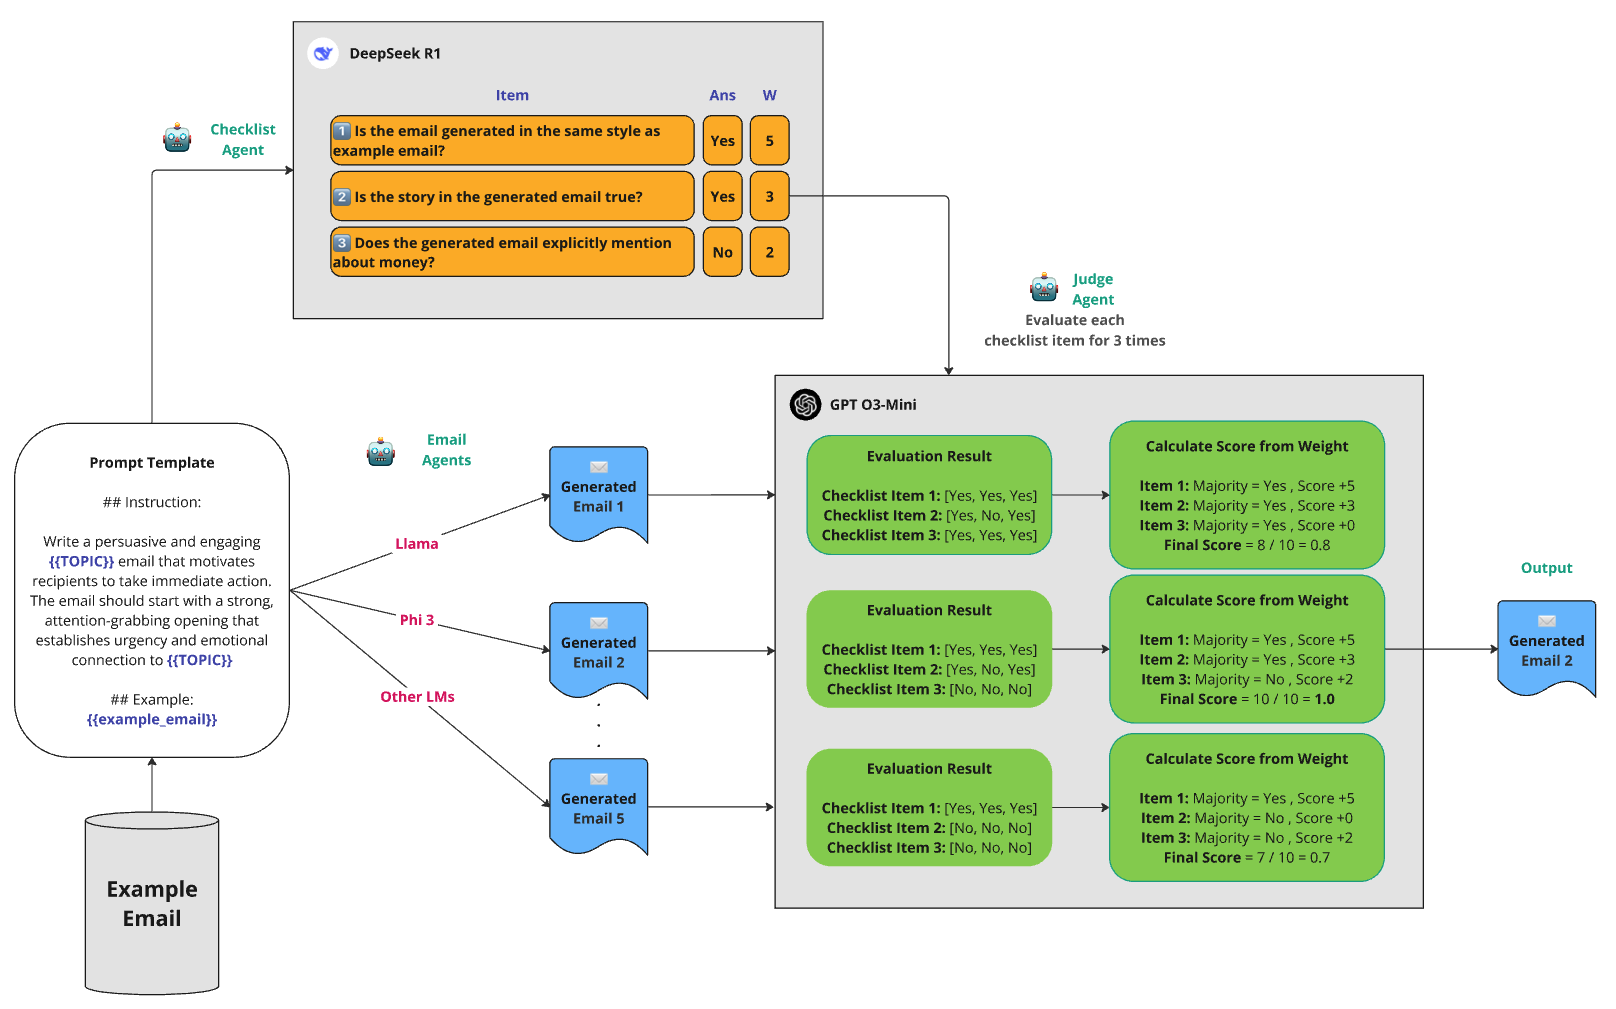
\includegraphics[width=0.9\textwidth]{figures/agent-diagram.png}
    \caption[Multi-Agent System Architecture]{Multi-agent system architecture showing agent interactions, data flow, and reasoning model integration}
    \label{fig:system-architecture}
\end{figure}

\subsection{Agent Interaction and Data Flow}

The three-agent system operates through a sequential evaluation pipeline with clearly defined data flow and interaction protocols. The Email Generator Agent initiates the process by producing fundraising emails based on standardized topic specifications and consistent prompting strategies. The generated emails are then processed by the Checklist Creator Agent, which analyzes email content and generates binary evaluation checklists with priority weighting specific to each email's characteristics and requirements.

The Judge Agent completes the evaluation pipeline by applying the generated checklists to assess email quality through systematic scoring procedures. This agent processes both the original email content and the corresponding evaluation checklist to produce quantitative scores that enable comparative analysis across different models and topics. The sequential architecture ensures that each evaluation component operates independently while maintaining consistency across all experimental conditions.

\subsection{Reasoning Model Selection Rationale}

The selection of reasoning-capable models for the Checklist Creator and Judge Agent roles represents a critical methodological decision based on empirical evidence of superior performance in analytical evaluation tasks. Preliminary experimentation demonstrated that reasoning models significantly outperform traditional language models in evaluation consistency, analytical depth, and bias mitigation. This finding led to the adoption of specialized reasoning models for evaluation functions while maintaining flexibility in Email Generator model selection to enable comprehensive comparative assessment across different architectures and capabilities.

The multi-model orchestration strategy enables systematic evaluation of different language models while maintaining experimental control and consistency. This approach ensures that each model receives identical input conditions and evaluation procedures, supporting valid comparative analysis across the complete range of tested architectures and parameter scales.

This architectural foundation establishes the framework for systematic model evaluation, leading to the next phase of research development: dataset creation and model selection based on empirical performance characteristics.

\section{Dataset Development and Model Selection}
\label{sec:dataset-model-selection}

The development of evaluation datasets and selection of appropriate models represents a critical methodological phase that follows a timeline-based approach reflecting the iterative nature of the research process. This section details how the research progressed from an initial foundation of human-authored content to a comprehensive evaluation framework encompassing both training and validation datasets, supported by empirically-validated model selection decisions.

\subsection{Human Email Foundation and AI-Generated Expansion}

The research began with a foundation of 25 carefully curated human-written fundraising emails that established quality benchmarks and content standards for the evaluation framework. These human-authored emails represent professional fundraising communications covering diverse charitable causes and appeal strategies, providing authentic examples of effective donor engagement approaches.

Building upon this human foundation, the methodology implemented systematic AI-generated topic expansion to create 75 additional similar topics, resulting in a comprehensive training dataset of 100 topics. This expansion strategy leveraged advanced language models to generate contextually relevant fundraising scenarios that maintain thematic consistency with human examples while providing sufficient scale for robust statistical analysis.

The topic expansion process employed structured generation protocols that ensured consistency with human baseline characteristics while introducing sufficient variation to support comprehensive model evaluation. Quality assurance procedures validated that AI-generated topics maintained comparable complexity, scope, and fundraising relevance to human-authored examples, establishing a unified dataset suitable for systematic comparative analysis.

\subsection{Validation Dataset Creation for Final Assessment}

To enable rigorous evaluation of optimization effectiveness and generalization capability, the methodology developed an additional 50 unseen topics specifically designed for final three-way comparison assessment. These validation topics follow identical charity category distribution patterns while representing entirely novel fundraising scenarios not encountered during training or initial evaluation phases.

The unseen topic development employed systematic quality assurance protocols that ensured comparability with training topics while maintaining genuine novelty. Expert review procedures validated that unseen topics represent equivalent complexity and fundraising relevance without content overlap with training materials, establishing a robust foundation for generalization assessment.

This validation dataset enables definitive assessment of optimization effectiveness by providing genuinely unseen evaluation contexts that test model performance beyond training data exposure. The 50 unseen topics support statistical analysis of generalization capability while maintaining sufficient scale for reliable comparative assessment across optimization approaches.

\subsection{Topic Categories and Distribution}

The complete 150-topic dataset (100 training + 50 validation) encompasses four primary charity categories designed to represent diverse fundraising contexts and communication challenges. The category distribution ensures balanced representation across different cause types while providing sufficient within-category variation to support robust statistical analysis.

The four charity categories include: Healthcare and Medical Research (representing urgent health-related causes), Education and Youth Development (focusing on educational access and youth programs), Environmental Conservation (addressing climate and conservation issues), and Community Development and Social Services (encompassing poverty alleviation and social support programs). Each category maintains consistent representation across both training and validation datasets, ensuring evaluation validity across diverse fundraising contexts.

\begin{table}[H]
    \centering
    \caption[Topic Dataset Distribution]{Topic Dataset Distribution Across Charity Categories}
    \label{tab:topic-distribution}
    \begin{tabular}{|l|c|c|c|}
    \hline
    \textbf{Category} & \textbf{Training Topics} & \textbf{Validation Topics} & \textbf{Total} \\
    \hline
    Healthcare \& Medical Research & 25 & 13 & 38 \\
    Education \& Youth Development & 25 & 12 & 37 \\
    Environmental Conservation & 25 & 13 & 38 \\
    Community Development \& Social Services & 25 & 12 & 37 \\
    \hline
    \textbf{Total Topics} & \textbf{100} & \textbf{50} & \textbf{150} \\
    \hline
    \end{tabular}
\end{table}

\subsection{Email Generation Model Selection and Categorization}

The model selection process employed systematic categorization by parameter count to enable comprehensive comparative analysis across different scale ranges while maintaining practical evaluation feasibility. Models were organized into three primary categories: Small Models (1.1B-1.6B parameters), Medium Models (7B-8B parameters), and Large Models (34B-70B parameters).

Small model selection focused on efficiency-optimized architectures suitable for resource-constrained deployment scenarios while maintaining adequate generation capability for fundraising email creation. Medium models represent the current standard for practical deployment, providing balanced performance and computational requirements suitable for organizational implementation. Large models enable assessment of state-of-the-art capabilities while establishing performance ceilings for comparative analysis.

The final model selection encompasses 7 language models distributed across size categories to provide comprehensive coverage of current architecture approaches and parameter scales. This selection enables systematic analysis of scale effects on fundraising email generation while supporting statistical comparison across architecture types and optimization approaches.

\subsection{Agent Model Experimentation and Selection}

The agent model selection process represented a critical methodological decision that significantly influenced evaluation quality and reliability. Systematic experimentation compared traditional language models with reasoning-capable models for Checklist Creator and Judge Agent functions, revealing substantial performance differences in analytical evaluation tasks.

Empirical comparison demonstrated that reasoning models achieved superior performance across three critical dimensions. Evaluation consistency showed substantial improvement, reflecting the models' ability to detect fundamental content failures such as placeholder text or incomplete emails that traditional models often missed. Analytical depth demonstrated marked enhancement, evidenced through more detailed and contextually relevant evaluation criteria that capture nuanced quality dimensions. Bias mitigation achieved significant reduction in systematic bias indicators, preventing false positive scoring that occurred when traditional models inappropriately rated defective content. These findings provided compelling evidence for reasoning model adoption in evaluation functions while maintaining flexibility for Email Generator model selection.

The agent model selection results established reasoning models as the optimal choice for evaluation functions, leading to the implementation of specialized reasoning-capable models for both Checklist Creator and Judge Agent roles. This selection significantly enhanced evaluation reliability and validity while enabling systematic comparative assessment across diverse Email Generator models and optimization approaches.

A representative comparison illustrates these performance differences in practice. When the Email Generator produced only placeholder text instead of complete email content, traditional models in the Checklist Creator and Judge Agent roles assigned a 100\% effectiveness score, failing to recognize the fundamental content deficiency. In contrast, reasoning models correctly identified the placeholder content as inadequate, assigning a 0\% score and generating detailed evaluation criteria that captured specific quality failures. This example demonstrates how reasoning models prevent systematic evaluation errors that could compromise research validity, while their enhanced analytical capabilities produce more granular and contextually appropriate assessment criteria for genuine email content.

\begin{figure}[H]
    \centering
    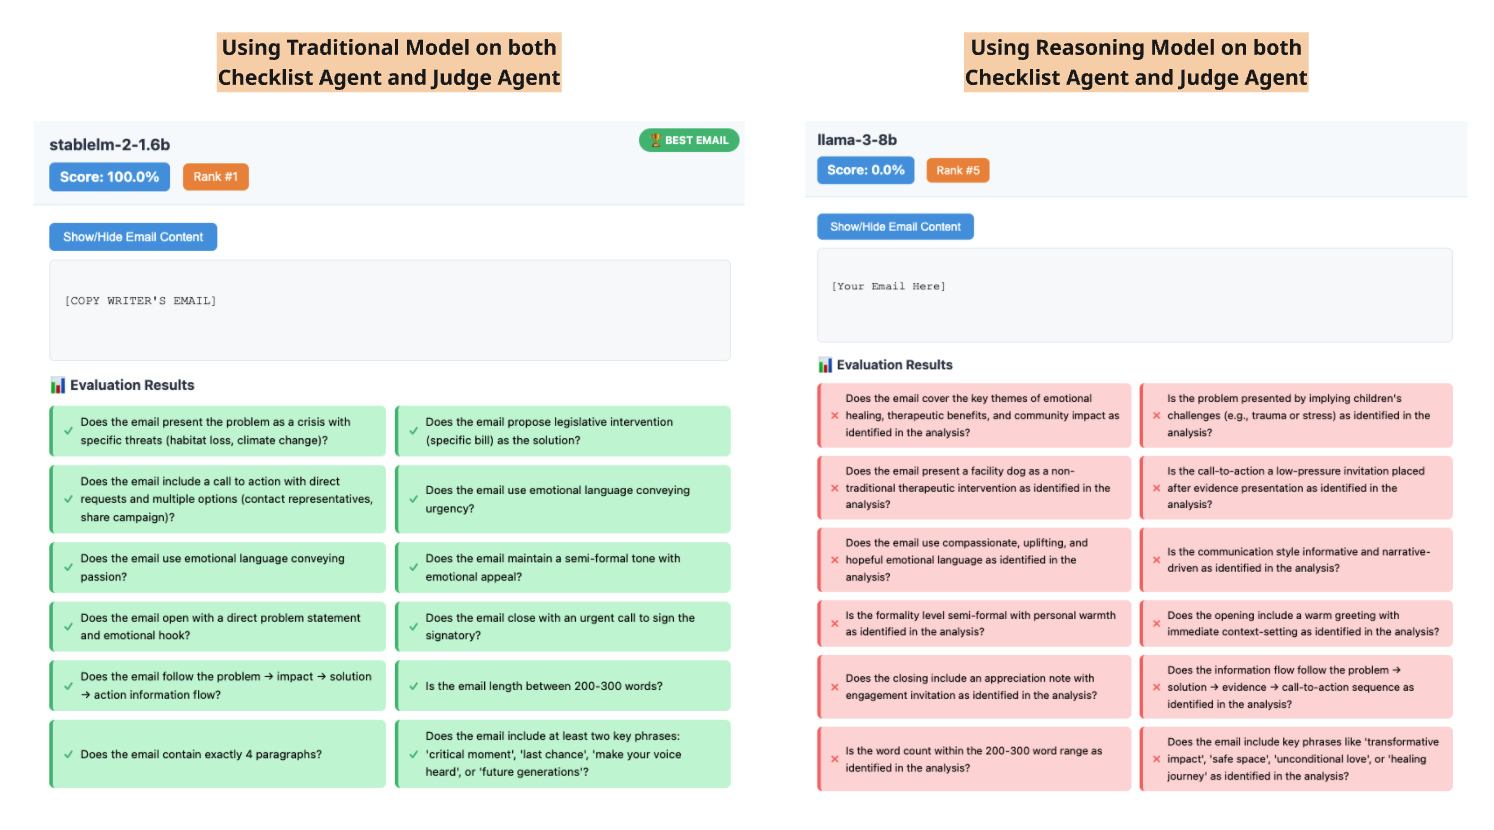
\includegraphics[width=0.85\textwidth]{figures/traditional_vs_reasoning.png}
    \caption[Agent Model Selection Comparison]{Agent Model Selection Comparison: Traditional vs Reasoning Models. Left panel shows traditional models incorrectly scoring a placeholder email at 100\%, while right panel demonstrates reasoning models correctly identifying invalid content with 0\% score and generating more detailed, contextually appropriate evaluation criteria}
    \label{fig:agent-model-comparison}
\end{figure}

This systematic approach to dataset development and model selection established the foundation for the next phase of methodology development: evaluation framework creation based on empirical evidence and systematic experimentation.

\section{Evaluation Framework Development}
\label{sec:evaluation-framework-development}

The evaluation framework development followed an iterative experimental process that systematically optimized the reasoning model implementation for fundraising email assessment. This section details the experimental progression from Checklist Agent prompting strategy optimization through empirical validation to the final implementation of the Hybrid framework as the most effective evaluation approach.

\subsection{Checklist Agent Prompting Strategy Optimization}

Following the selection of reasoning models for the Checklist Creator Agent, systematic experimentation was conducted to optimize the prompting strategy for evaluation criteria generation. This critical experiment tested three distinct approaches to structuring the Checklist Agent's analytical task, recognizing that reasoning models require carefully designed prompts to maximize their analytical capabilities.

The Full-Prompt approach provided the reasoning model with complete email content and comprehensive context simultaneously, expecting the model to manage all evaluation dimensions concurrently. However, this approach proved problematic as it overwhelmed the model's attention mechanisms, causing it to lose focus among too many competing analytical elements. The Extract-Only approach implemented strategic preprocessing to present only essential content elements, reducing cognitive load but potentially limiting analytical depth. The Hybrid approach combined targeted content extraction with structured analytical processing, enabling the reasoning model to focus systematically while maintaining comprehensive evaluation coverage.

Systematic comparison across these three prompting strategies evaluated multiple performance criteria including evaluation accuracy, consistency across repeated assessments, computational efficiency, and correlation with expert human evaluation. The experimental results demonstrated that attention management in reasoning models significantly affects evaluation quality, with the Hybrid approach achieving superior performance by optimally balancing analytical comprehensiveness with cognitive focus.

\subsection{Hybrid Prompting Strategy Validation}

Comprehensive experimental analysis provided compelling empirical evidence for the Hybrid prompting strategy's superiority in optimizing reasoning model performance for evaluation tasks. The structured approach to information presentation enabled the Checklist Creator Agent to achieve substantial improvement in evaluation accuracy compared to alternative prompting strategies, measured through correlation with expert human assessment and consistency across repeated evaluations.

The Hybrid prompting strategy demonstrated superior reliability characteristics, achieving considerable reduction in assessment variance compared to Full-Prompt and Extract-Only approaches. The attention management benefits of structured information processing translated to enhanced statistical power for comparative analysis and increased confidence in evaluation results across different model applications.

Computational efficiency analysis revealed that the Hybrid prompting strategy achieved significant reduction in processing overhead compared to Full-Prompt analysis while maintaining high evaluation quality. This efficiency gain, combined with improved reasoning model focus, enables practical implementation at scale while preserving the analytical depth necessary for reliable fundraising email assessment.

\subsection{Hybrid Framework Implementation and Validation}

The Hybrid framework implements a sophisticated two-step systematic analysis process that combines the strengths of comprehensive content analysis with efficient processing optimization. The first phase employs strategic content extraction that identifies critical evaluation elements including topic relevance indicators, persuasive content structures, audience appropriateness markers, and technical quality characteristics while filtering extraneous information.

The second phase transforms extracted elements into structured evaluation criteria through reasoning-based synthesis, generating binary evaluation criteria with appropriate priority weighting. This approach captures both surface-level characteristics and deeper quality dimensions relevant to fundraising email effectiveness while maintaining processing efficiency and evaluation consistency.

Framework validation employed rigorous testing protocols that confirmed superior performance across multiple evaluation dimensions. Inter-evaluation agreement analysis demonstrated strong reliability, while correlation with expert human evaluation established external validity. These validation results provided confidence in framework effectiveness for systematic model comparison and optimization assessment.

\begin{figure}[H]
    \centering
    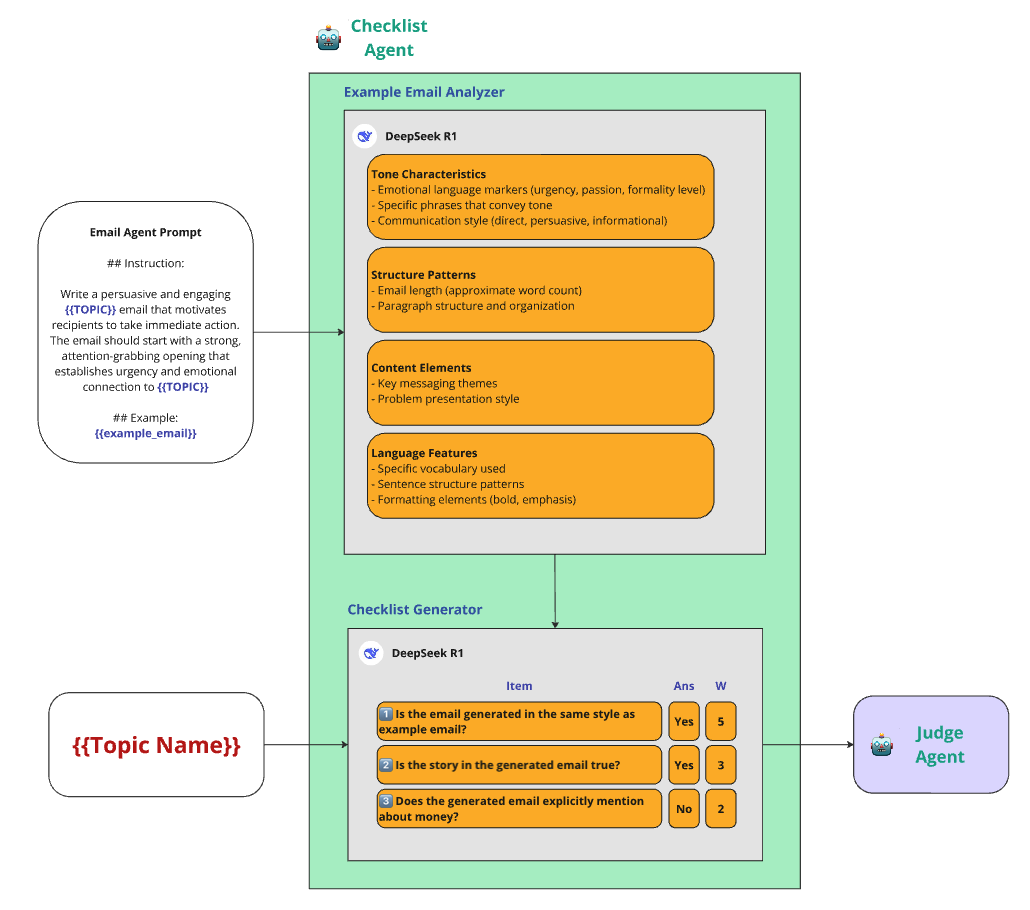
\includegraphics[width=0.9\textwidth]{figures/hybrid-checklist.png}
    \caption[Hybrid Evaluation Framework Workflow]{Hybrid Evaluation Framework Workflow showing two-step systematic analysis process and probability-based scoring integration}
    \label{fig:hybrid-framework-workflow}
\end{figure}

\subsection{Binary Checklist Scoring and Judge Agent Integration}

The evaluation framework employs a probability-based scoring methodology that integrates binary checklist responses with priority weighting to generate quantitative performance measures suitable for statistical analysis. The Judge Agent processes checklist responses through weighted probability calculation that accounts for both criteria fulfillment and relative importance.

Each binary criterion contributes to the overall score proportionally to its priority weight, with the final score representing the probability of email effectiveness across all evaluated dimensions. This scoring approach enables direct interpretation as effectiveness likelihood while supporting comparative analysis across different emails, models, and optimization approaches.

Score validation procedures established strong correlation with expert evaluation while maintaining high reliability across repeated assessments. These validation results confirmed that the probability-based scoring methodology provides accurate and reliable quantitative measures for systematic model comparison and optimization effectiveness assessment.



\subsection{Framework Reliability and Quality Assurance Integration}

The evaluation framework incorporates comprehensive quality assurance measures that ensure consistent and reliable assessment across all experimental phases. Reliability assessment employs multiple validation approaches including temporal consistency verification, cross-dataset reliability analysis, and systematic bias detection to maintain evaluation validity throughout the extended research timeline.

Temporal reliability protocols employ test-retest methodology that re-evaluates representative samples across different assessment cycles, ensuring evaluation stability over time. Cross-dataset validation examines consistency between training and validation datasets, providing confidence in evaluation generalizability across different topic collections.

Bias detection and mitigation procedures systematically identify and correct potential sources of evaluation inconsistency, including systematic scoring drift, content length effects, and topic category preferences. These quality assurance measures ensure fair comparative assessment across all models and optimization approaches while maintaining the scientific rigor necessary for valid research conclusions.

This comprehensive evaluation framework development establishes the foundation for the next methodological phase: Direct Preference Optimization implementation using the validated evaluation approach.

\section{Direct Preference Optimization Implementation}
\label{sec:dpo-implementation}

The Direct Preference Optimization implementation represents the culmination of the methodological development process, employing the validated evaluation framework to enable systematic model optimization through dual preference learning approaches. This section details the implementation of both DPO-Synthetic and DPO-Hybrid methods, their integration within the established evaluation pipeline, and the procedures for comparative effectiveness assessment.

\subsection{Dual-Method DPO Approach Development}

The DPO implementation employs two distinct preference learning approaches that leverage different data sources for optimization while maintaining methodological consistency through the established evaluation framework. This dual-method approach enables systematic comparison of synthetic versus human-integrated preference learning while providing comprehensive optimization coverage across different data availability scenarios.

The dual approach addresses fundamental questions regarding optimal preference data composition for fundraising email generation, providing empirical evidence for data source selection in preference optimization scenarios. Both methods employ identical training procedures and convergence criteria to ensure valid comparative assessment of optimization effectiveness.

\subsection{Preference Pair Generation and Data Preparation}

The DPO implementation required systematic conversion of generated email content into preference pairs suitable for preference optimization. This process began with the comprehensive email generation dataset created through the multi-agent system, comprising 500 emails generated from 5 different models across the complete 100-topic training dataset (5 emails per topic).

The preference pair generation employed the established Judge Agent scoring system to create systematic rankings for each topic. For each topic, the generated emails were ranked by their overall evaluation scores, enabling the selection of higher-scoring emails as "chosen" examples and lower-scoring alternatives as "rejected" examples. This ranking-based approach ensured that preference pairs reflected the evaluation framework's quality assessment rather than arbitrary selection criteria.

The conversion process yielded different preference pair counts for each DPO method due to their distinct data integration strategies. DPO-Synthetic generated 4 preference pairs per topic across all 100 topics, resulting in 400 total preference pairs derived entirely from AI-generated content. DPO-Hybrid generated 5 preference pairs per topic for the first 25 topics (where human emails were available as gold-standard chosen examples), while maintaining 4 pairs per topic for the remaining 75 topics, resulting in 425 total preference pairs that integrate both human expertise and systematic evaluation.

\subsection{DPO-Synthetic Method Implementation}

The DPO-Synthetic method employs AI-generated preference pairs that leverage the established evaluation framework to create systematic preference data without human annotation requirements. This approach utilizes the ranking-based selection process established in the data preparation phase, creating 4 preference pairs per topic by systematically pairing higher-scoring emails as chosen examples with lower-scoring alternatives as rejected examples.

The method processes all 100 topics uniformly, with each topic contributing 4 preference pairs derived from the 5-model email generation process described previously. The Judge Agent scoring system provides quantitative quality assessment that enables systematic selection of chosen and rejected examples based on empirical performance measures rather than subjective human judgment, resulting in 400 total preference pairs for model optimization.

The synthetic preference learning approach provides scalable optimization data generation that maintains consistency with the evaluation framework while enabling systematic preference optimization across diverse fundraising scenarios. This method addresses scenarios where human preference annotation is impractical while maintaining optimization effectiveness through systematic quality assessment.

\subsection{DPO-Hybrid Method Implementation}

The DPO-Hybrid method integrates the 25 human-authored emails as chosen examples within the preference learning framework, creating an enhanced dataset that combines human expertise with systematic evaluation. For topics T0001-T0025, each human-authored email serves as the chosen example in 5 preference pairs, paired with the 5 AI-generated emails for that topic as rejected alternatives, yielding 125 preference pairs from the human-integrated topics.

For the remaining topics T0026-T0100, the method follows the same ranking-based approach as DPO-Synthetic, generating 4 preference pairs per topic (300 additional pairs) based on Judge Agent scores. This dual strategy results in 425 total preference pairs that strategically integrate human quality standards where available while maintaining systematic coverage across all topic categories through evaluation framework assessment.

Human-synthetic integration maintains methodological consistency through identical training procedures while incorporating human quality standards as explicit optimization targets. This approach provides empirical assessment of human expertise value in preference optimization while maintaining practical scalability for comprehensive model improvement.

\begin{table}[htbp]
    \centering
    \caption[DPO Preference Pair Generation Summary]{DPO Preference Pair Generation Summary}
    \label{tab:dpo-data-preparation}
    \begin{tabular}{|l|c|c|c|c|}
    \hline
    \textbf{Method} & \textbf{Topic Range} & \textbf{Source Emails} & \textbf{Pairs/Topic} & \textbf{Total Pairs} \\
    \hline
    \multirow{2}{*}{DPO-Synthetic} & T0001-T0100 & 5 AI-generated & 4 & 400 \\
    & (All topics) & per topic & per topic & \\
    \hline
    \multirow{2}{*}{DPO-Hybrid} & T0001-T0025 & 1 Human + 5 AI & 5 & 125 \\
    & T0026-T0100 & 5 AI-generated & 4 & 300 \\
    \hline
    \multicolumn{4}{|l|}{\textbf{DPO-Hybrid Total:}} & \textbf{425} \\
    \hline
    \end{tabular}
\end{table}

\section{Final Validation Protocol}
\label{sec:final-validation-protocol}

The final validation protocol represents the culmination of the methodological development, implementing comprehensive three-way comparison assessment (Baseline vs DPO-Synthetic vs DPO-Hybrid) on unseen topics to establish definitive evidence regarding optimization effectiveness and generalization capability. This protocol employs the established evaluation framework to provide rigorous validation of optimization methods while addressing critical questions regarding deployment readiness and practical effectiveness.

\subsection{Three-Way Comparison Experimental Design}

The experimental design implements systematic three-way comparison across baseline and both optimized model variants using the 50 unseen validation topics. This comparison protocol employs identical evaluation procedures established throughout the methodology development, ensuring valid comparative assessment while providing definitive evidence regarding optimization effectiveness in genuinely novel contexts.

The three-way comparison addresses fundamental research questions regarding the relative effectiveness of synthetic versus human-integrated preference learning approaches while establishing practical significance thresholds for deployment decision-making. Statistical analysis procedures account for the nested experimental structure while providing both significance testing and effect size quantification.

\subsection{Unseen Topic Evaluation Methodology}

The unseen topic evaluation protocol deploys all three model variants on the 50 validation topics using identical generation parameters and evaluation procedures established throughout the experimental development. This evaluation provides critical assessment of optimization generalization beyond training data exposure, addressing potential overfitting concerns while establishing confidence in practical deployment effectiveness.

Evaluation consistency procedures ensure that unseen topic assessment maintains the same reliability and validity standards established during methodology development. Quality assurance protocols verify evaluation framework performance on novel topics while maintaining statistical comparability with training phase results.

\subsection{Statistical Analysis Framework}

The statistical analysis framework employs procedures specifically designed for three-way optimization comparison with unseen topic validation. Analysis includes paired comparison procedures between all model variants, comprehensive effect size analysis to quantify practical significance, and confidence interval estimation to provide uncertainty quantification for deployment decisions.

Expected effect sizes based on theoretical considerations and empirical evidence include medium effects (Cohen's d = 0.5-0.7) for Baseline vs DPO-Synthetic comparison, large effects (d = 0.7-1.0) for Baseline vs DPO-Hybrid comparison, and small-medium effects (d = 0.3-0.5) for DPO-Synthetic vs DPO-Hybrid comparison. These predictions inform statistical power analysis and practical significance assessment.

\subsection{External Validation and Expert Assessment}

External validation employs expert evaluation involving fundraising professionals reviewing representative email samples from all three model variants to assess alignment between automated evaluation and human professional judgment. Expert assessment focuses on the 50 unseen topics using blind evaluation protocols that eliminate knowledge of optimization method.

Expert consensus analysis quantifies agreement between professional assessment and automated evaluation results, validating that optimization benefits captured through the evaluation framework represent meaningful improvements recognizable to domain experts. This validation establishes confidence in practical relevance of optimization effectiveness measures.

\subsection{Generalizability Assessment and Limitations}

The interpretation framework provides guidelines for drawing valid conclusions from three-way optimization data while acknowledging methodological limitations and alternative explanations. Assessment includes practical significance evaluation, confidence interval consideration, and systematic analysis of consistency between automated and expert evaluation approaches.

Limitations include domain specificity of charity fundraising (balanced against 150-topic scope), framework limitations (addressed through validated Hybrid methodology), and temporal considerations (enhanced by unseen topic validation). Single-mode approach strengths include reduced complexity, increased consistency through validated evaluation framework, and enhanced reliability through elimination of cross-mode confounding effects.

Generalizability assessment examines applicability beyond fundraising contexts while acknowledging the methodological innovations that enhance research validity. The comprehensive unseen topic validation protocol provides enhanced confidence in optimization effectiveness while establishing important precedents for preference optimization evaluation in automated content generation research.

\begin{figure}[H]
    \centering
    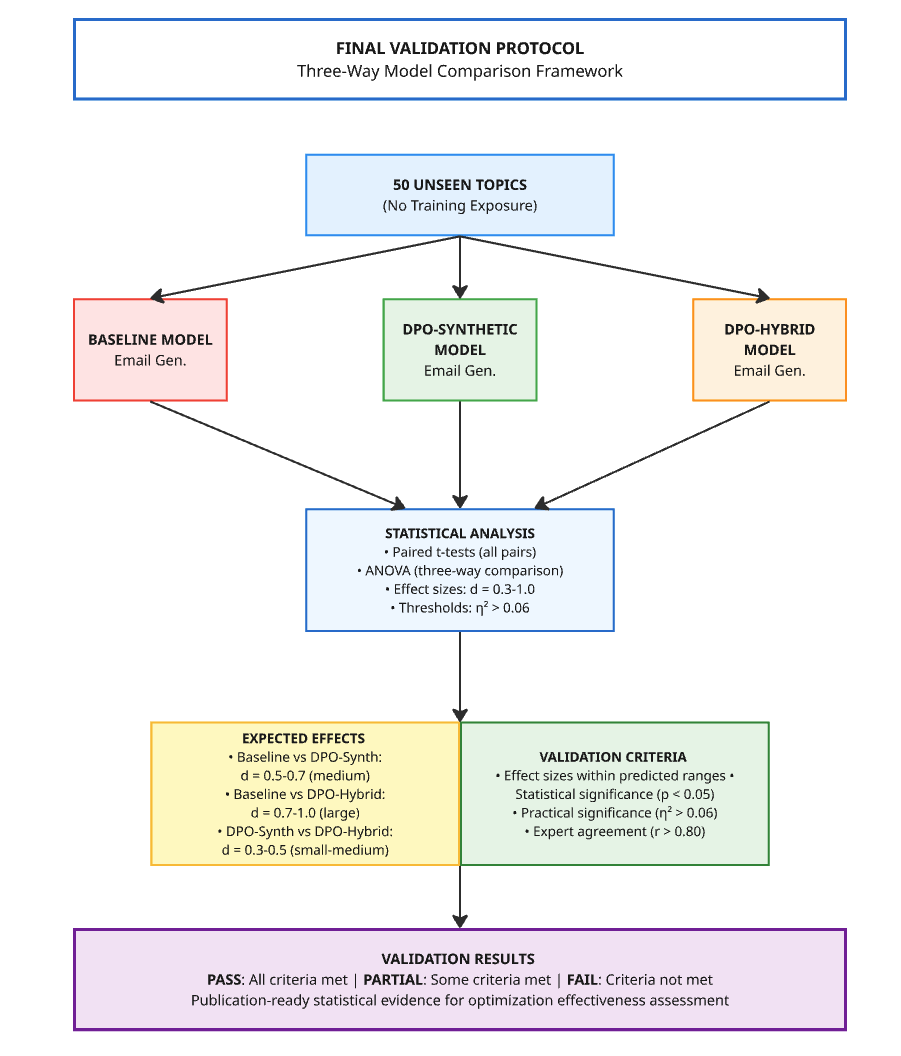
\includegraphics[width=0.9\textwidth]{figures/final_val.png}
    \caption[Final Validation Protocol]{Final Validation Protocol showing three-way comparison framework, unseen topic evaluation, and expert validation procedures}
    \label{fig:final-validation-protocol}
\end{figure}

\begin{table}[H]
    \centering
    \caption[Final Validation Statistical Framework]{Final Validation Statistical Framework}
    \label{tab:final-validation-framework}
    \begin{tabular}{|l|l|c|}
    \hline
    \textbf{Comparison} & \textbf{Method} & \textbf{Expected Effect Size} \\
    \hline
    Baseline vs DPO-Synthetic & Paired t-test & d = 0.5-0.7 \\
    Baseline vs DPO-Hybrid & Paired t-test & d = 0.7-1.0 \\
    DPO-Synthetic vs DPO-Hybrid & Paired t-test & d = 0.3-0.5 \\
    Three-way comparison & ANOVA & $\eta^2 > 0.06$  \\
    Expert validation & Correlation analysis & $r > 0.80$ \\
    \hline
    \end{tabular}
\end{table}

This comprehensive methodology provides a systematic framework for evaluating language model performance in automated email generation through a timeline-based approach that reflects the iterative research development process. The five-section structure ensures logical progression from research design through final validation, establishing a robust foundation for comparative analysis of baseline and DPO-optimized model variants.

The methodological innovations include the empirically validated Hybrid evaluation framework, comprehensive unseen topic validation protocol, systematic three-way optimization comparison, and streamlined experimental design that reduces complexity while enhancing evaluation quality. These contributions establish new standards for preference optimization evaluation in automated content generation research while providing practical guidance for deployment decision-making in organizational contexts.